\section{Commercial LCR meters} \label{sec:CommercialLCRMeters}
Most of the major manufacturers of test equipment, such as Keysight Technologies, Rohde \& Schwarz, Tektronix and others produce a range of instruments for characterizing passive components. This section will review a few of these to find out what their capabilities are. 

LCR meters typically come in two different form factors, one is a handheld device, much like a regular multimeter, while the other is a benchtop instrument. The handheld LCR meters, like the Keysight U1733C\cite{KeysightU1733C} shown on figure \ref{fig:2_2_U1733C}.
\begin{figure}[H]
    \centering
    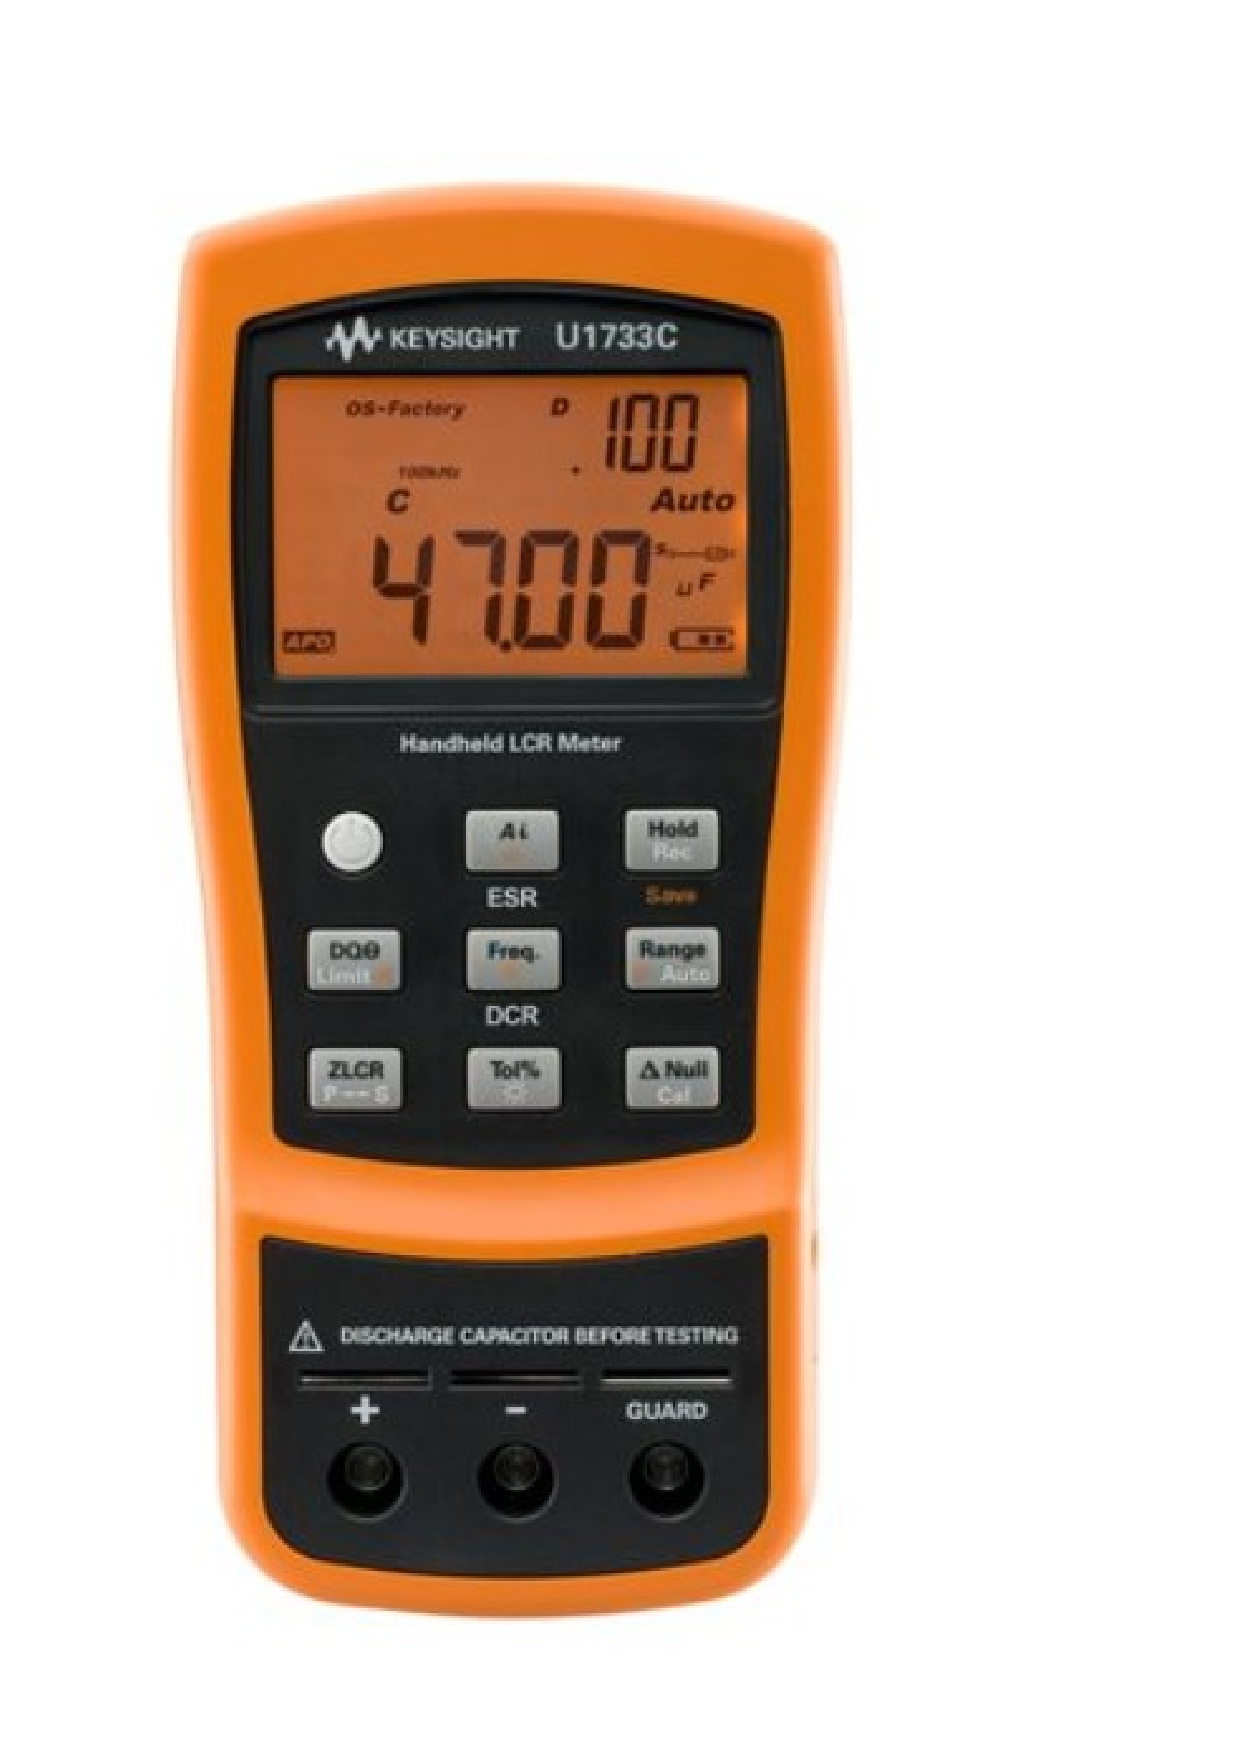
\includegraphics[clip, trim=0 50 0 50, width=0.5\textwidth]{Sections/2_ProblemAnalysis/FIgures/KeysightU1733C.pdf}
    \caption{A handheld Keysight U1733C LCR meter.\cite{KeysightU1733C}}
    \label{fig:2_2_U1733C}
\end{figure}
The U1733C \ref{fig:2_2_U1733C}, while affordable at about 550€, has limited capabilities. It can measure all the basic parameters such as capacitance, inductance, ESR and display all the derived quantities like dissipation and quality factor numerically, however it can only take these measurements at a pre-determined set of test frequencies in the range \SI[]{100}{\hertz} to \SI[]{100}{\kilo\hertz} with measurement accuracy weaning off in both ends of the frequency range as shown on figure \ref{fig:2_2_U1733CCapAccurancy}.

\begin{figure}[H]
    \centering
    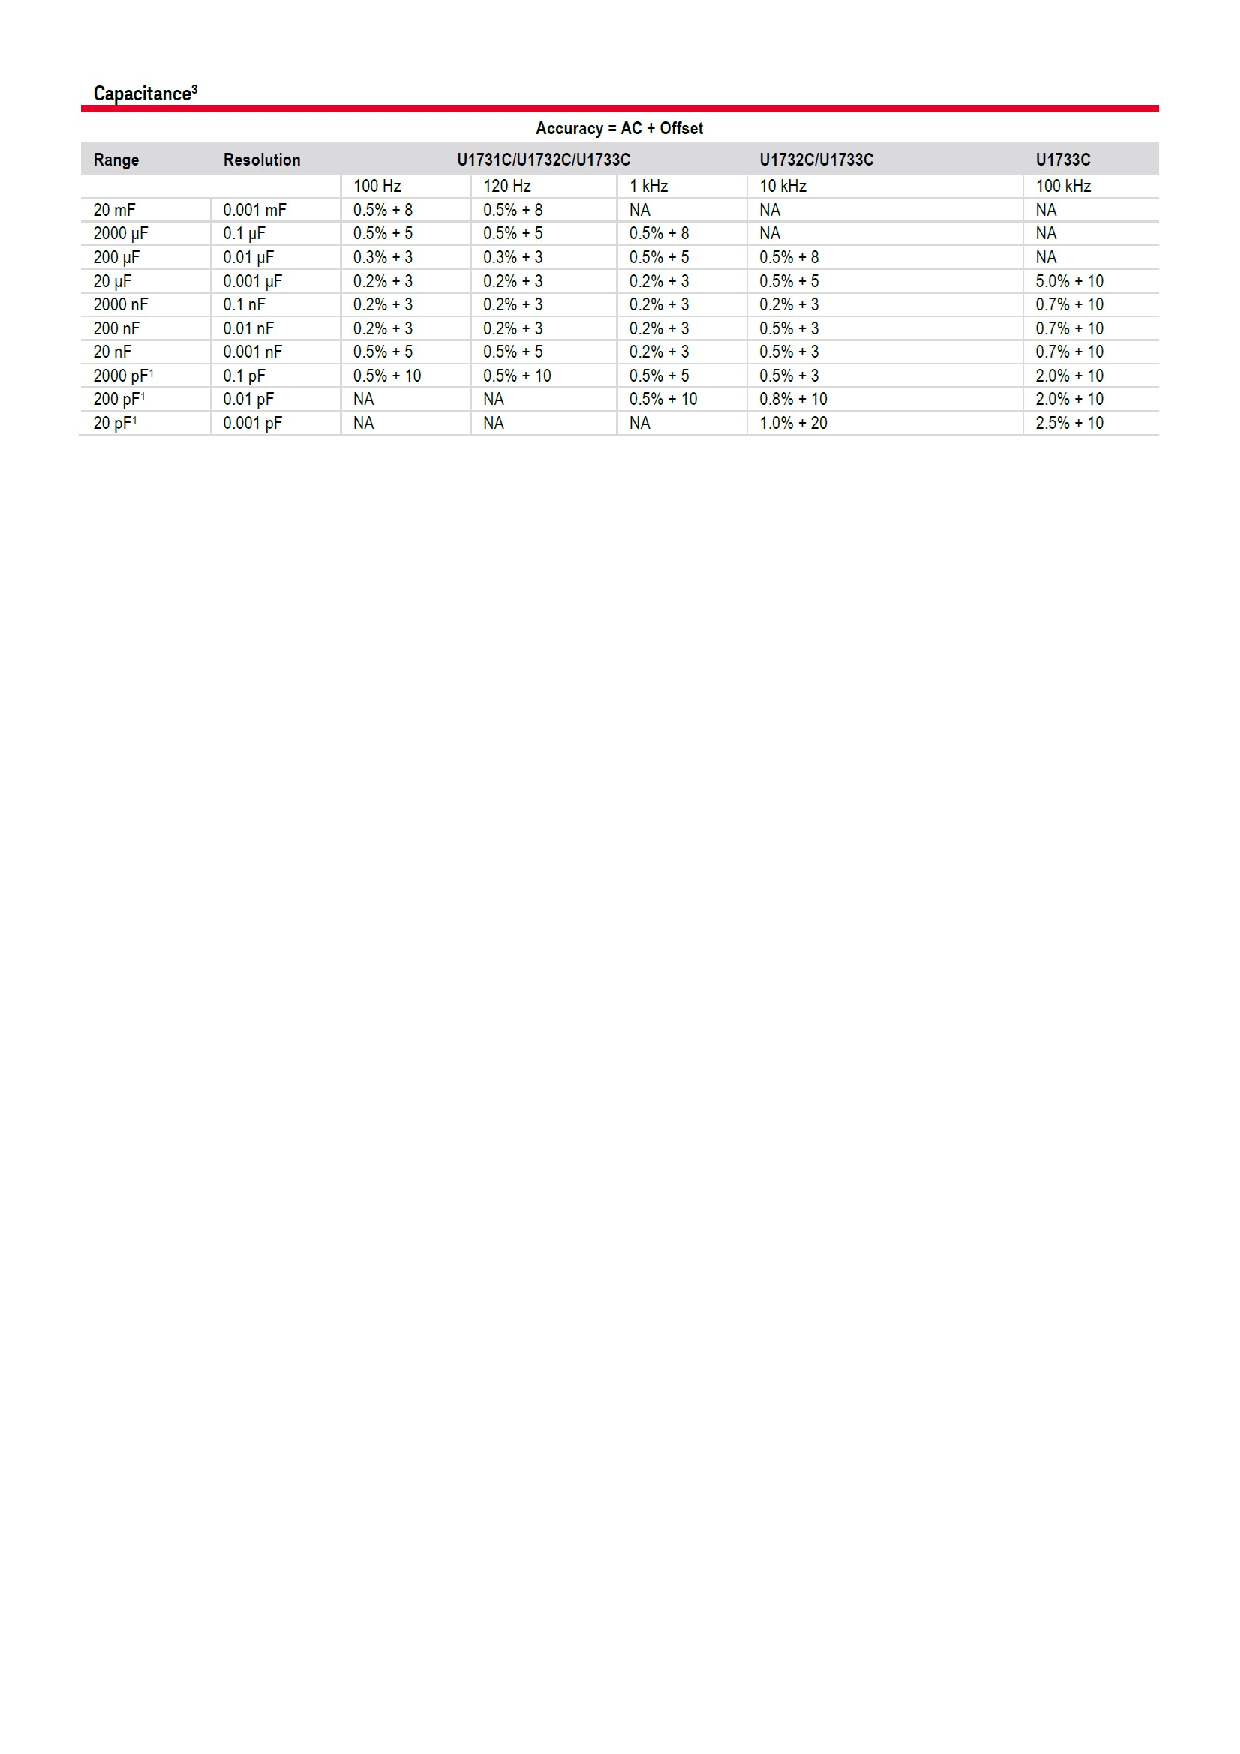
\includegraphics[clip, trim=0 630 0 0, width=1\textwidth]{Sections/2_ProblemAnalysis/FIgures/U1733CAccuracyDatasheet.pdf}
    \caption{A snapshop from the Keysight U1733C datasheet listing the accuracy of capacitance measurements.\cite{KeysightU1733CDatasheet}. Measurements for inductance, resistance and so on show a similar pattern.}
    \label{fig:2_2_U1733CCapAccurancy}
\end{figure}

The U1733C datasheet has similar charts for other measurements, but they follow a similar pattern of accuracy as capacitance where it becomes clear that the accuracy is worse in the higher ends of the range. The accuracy is listed as a $\%$ of range $ + n\cdot resolution$, so a measurement in the \SI[]{20}{\micro\farad} range will have an accuracy of $\pm \SI[]{1}{\micro\farad} + \SI[]{10}{\nano\farad}$





%Vi kigger kun på bord LCR metre

%VI kigger på 3 forskellige
%Keysight
%RS
%Tek

%De har xyz specs og kan de her ting.

%De er beregnet til xyz

%de koster xyz

